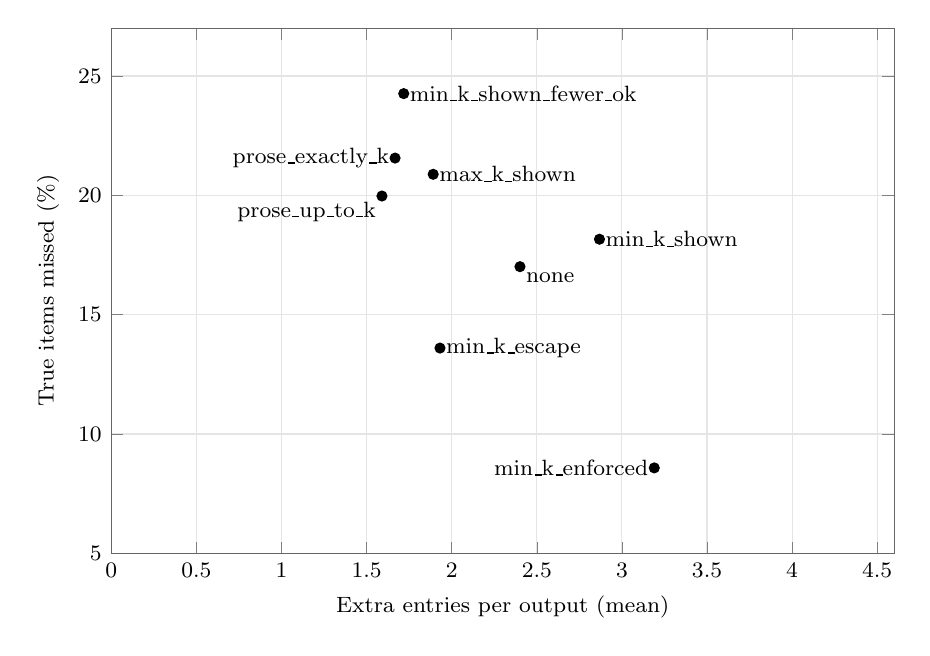
\begin{tikzpicture}
\begin{axis}[scale only axis, width=0.82\columnwidth, height=0.55\columnwidth,
  xmin=0, xmax=4.6, ymin=5, ymax=27, grid=major, grid style={gray!20}, axis line style={black!60},
  xlabel={Extra entries per output (mean)}, ylabel={True items missed (\%)},
  label style={font=\footnotesize}, tick label style={font=\footnotesize}]
\addplot[only marks, mark=*, mark size=1.8pt, color=black] coordinates {(2.401,17.01) (1.590,19.97) (1.667,21.56) (1.891,20.88) (2.868,18.16) (1.718,24.26) (3.190,8.58) (1.931,13.60)};
\node[font=\footnotesize, anchor=north west, inner sep=2pt] at (axis cs:2.401,17.01) {\cnd{none}};
\node[font=\footnotesize, anchor=north east, inner sep=2pt] at (axis cs:1.590,19.97) {\cnd{prose\_up\_to\_k}};
\node[font=\footnotesize, anchor=east, inner sep=2pt] at (axis cs:1.667,21.56) {\cnd{prose\_exactly\_k}};
\node[font=\footnotesize, anchor=west, inner sep=2pt] at (axis cs:1.891,20.88) {\cnd{max\_k\_shown}};
\node[font=\footnotesize, anchor=west, inner sep=2pt] at (axis cs:2.868,18.16) {\cnd{min\_k\_shown}};
\node[font=\footnotesize, anchor=west, inner sep=2pt] at (axis cs:1.718,24.26) {\cnd{min\_k\_shown\_fewer\_ok}};
\node[font=\footnotesize, anchor=east, inner sep=2pt] at (axis cs:3.190,8.58) {\cnd{min\_k\_enforced}};
\node[font=\footnotesize, anchor=west, inner sep=2pt] at (axis cs:1.931,13.60) {\cnd{min\_k\_escape}};
\end{axis}
\end{tikzpicture}
